% !TeX program = lualatex
% !TeX root = luaking.tex
% !TeX encoding = UTF-8
% !TeX spellcheck = cs_CZ
%---------------------------------------------------------------------------------------------------
% file fey1ch33.tex
%---------------------------------------------------------------------------------------------------
%=========================== Kapitola: Polarizace =================================================
\setchaptertoc
\chapter{Polarizace}\label{fyz:IchapXXXIII}
  \section{Elektrický vektor světla}\label{fyz:IchapXXXIIIsecI}
    V této kapitole se budeme zabývat jevy, jež souvisí s tím, že intenzita elektrického pole
    popisujícího světlo je vektor. V předcházejících kapitolách jsme se nezajímali o směr oscilací
    intenzity elektrického pole; pouze jsme poznamenali, že vektor intenzity elektrického pole leží
    v rovině kolmé ke směru šíření světla. Konkrétní směr, který v této rovině má, nás už nezajímal.
    Nyní si probereme jevy, jejichž hlavním rysem je právě konkrétní směr oscilací elektrického
    pole.

    V ideálním monochromatickém světle musí elektrické pole oscilovat s přesnou frekvencí, ale
    protože složka \(x\) a složka \(y\) oscilují nezávisle, musíme se podívat, co vznikne skládáním
    dvou nezávislých vzájemně kolmých oscilací. jaké pole vznikne, kmitají-li složka \(x\) i \(y\)
    se stejnou frekvencí? Probíhá-li kmitání ve směru osy \(x\) a k němu se přidá další kmitavý
    pohyb se stejnou fází ve směru osy \(y\), budou výsledné kmity probíhat v novém směru v rovině
    \(xy\). Na obr. \ref{fyz:fig0270} jsou znázorněny superpozice pro různé amplitudy kmitů \(x\) a
    \(y\). Výsledky znázorněné na obr. \ref{fyz:fig0270} nejsou jediné možné. Ve všech těchto
    případech jsme předpokládali, že kmity \(x\) a \(y\) jsou ve fázi, ale nemusí tomu tak být. Může
    se však stát, že kmity \(x\) a \(y\) nejsou ve fázi.

    Nejsou-li kmity \(x\) a \(y\) ve fázi, opisuje konec vektoru intenzity elektrického pole elipsu.
    Lze to znázornit známým způsobem. Zavěsíme-li kuličku na dlouhé vlákno tak, že se může volně
    kývat v horizontální rovině, bude vykonávat sinusoidální oscilace. Když umístíme počátek
    souřadnic \(x\) a \(y\) v klidové poloze kuličky, může kulička kmitat ve směru \(x\) nebo ve
    směru \(y\) se stejnou frekvencí kyvadla. Výběrem vhodné počáteční polohy a rychlosti můžeme
    docílit toho, že kulička kmitá buď podél osy \(x\) nebo podél osy \(y\) nebo podél libovolné
    přímky v rovině \(xy\) procházející počátkem. Tyto pohyby kuličky jsou analogické s oscilacemi
    vektoru intenzity elektrického pole znázorněnými na obr. \ref{fyz:fig0270}. Protože kmity \(x\) a
    \(y\) nabývají současně svá maxima a minima, jsou obě oscilace v každém okamžiku ve fázi. Víme
    však, že nejobecnější pohyb kuličky je pohyb po elipse; to odpovídá oscilacím, kdy pohyby \(x\)
    a \(y\) nejsou ve fázi. Superpozice kmitů \(x\) a \(y\), jež nejsou ve fázi, je znázorněna pro
    různé úhly mezi fázemi těchto kmitů na obr. \ref{fyz:fig0271}. Obecný výsledekje takový, že
    vektor intenzity elektrického pole opisuje elipsu. Pohyb po přímce je zvláštním případem pohybu
    po elipse, jenž odpovídá nulovému fázovému rozdílu (nebo celočíselnému násobku \(\pi\). Pohyb po
    kružnici odpovídá stejným amplitudám s fázovým rozdílem \ang{90} (nebo lichým celočíselným
    násobkům \(\pi/2\)).

    \begin{figure}[ht!]  %\ref{fyz:fig0270}
      \centering
      \subcaptionbox{\(E_y = 1\;  E_x = 0\)           \label{fyz:fig0270a}}
        {\luafigure[0.4]{fyz_fig0270a.pdf}}               
      \subcaptionbox{\(E_y = 1\;  E_x = \frac{1}{2}\) \label{fyz:fig0270b}}
        {\luafigure[0.4]{fyz_fig0270b.pdf}}                                                 \\
      \subcaptionbox{\(E_y = 1\;  E_x = 1\)           \label{fyz:fig0270c}}
        {\luafigure[0.4]{fyz_fig0270c.pdf}}                         
      \subcaptionbox{\(E_y = 0\;  E_x = 1\)           \label{fyz:fig0270d}}
        {\luafigure[0.4]{fyz_fig0270d.pdf}}                                                 \\         
      \subcaptionbox{\(E_y = 1\;  E_x = -1\)          \label{fyz:fig0270e}}
        {\luafigure[0.4]{fyz_fig0270e.pdf}}                         
      \subcaptionbox{\(E_y = -1\; E_x = 1\)           \label{fyz:fig0270f}}
        {\luafigure[0.4]{fyz_fig0270f.pdf}}
      \caption{Skládání kmitů ve směru os \(x\) a \(y\) ve fázi (\cite[s.~437]{Feynman01})}
      \label{fyz:fig0270}
    \end{figure}

    Na obr. \ref{fyz:fig0271} jsme označili vektory intenzity elektrického pole ve směrech \(x\) a
    \(y\) komplexními čísly, jež jsou vhodným způsobem pro vyjádření fázového rozdílu. Nezaměňujme
    přitom v tomto zápisu reálnou a imaginární složku komplexního elektrického vektoru se složkami
    pole \(x\) a \(y\). Složky \(x\) a \(y\) znázorněné na obr. \ref{fyz:fig0270} a obr.
    \ref{fyz:fig0271} jsou skutečná elektrická pole, která můžeme měřit. Reálná a imaginární složka
    komplexního vektoru intenzity elektrického pole jsou pouze vhodným matematickým vyjádřením a
    nemají fyzikální význam.

    Nyní trochu terminologie. Říkáme, že světlo je \textbf{lineárně polarizované} (někdy též rovinně
    polarizované), osciluje-li vektor intenzity elektrického pole podél přímky. Obrázek
    \ref{fyz:fig0270} znázorňuje lineární polarizaci. Pohybuje-li se konec vektoru intenzity
    elektrického pole po elipse, je světlo \textbf{elipticky polarizované}. Pohybuje-li se konec
    vektoru intenzity elektrického pole po kružnici, máme \textbf{kruhovou polarizaci}. Letí-li
    světlo přímo proti nám a konec vektoru elektrického pole se otáčí proti směru hodinových
    ručiček, jde o pravotočivou polarizaci. Obrázek \ref{fyz:fig0271g} znázorňuje
    \textbf{pravotočivou kruhovou polarizaci} a obrázek \ref{fyz:fig0271c}. Znázorňuje
    \textbf{levotočivou kruhovou polarizaci}. V obou případech světlo vychází kolmo ven z papíru.
    Naše konvence označování levotočivé a pravotočivé kruhové polarizace je konzistentní s
    označováním, které se dnes používá ve fyzice pro všechny další částice, jež projevují polarizaci
    (například elektrony). V některých knihách o optice se však používá opačná konvence, takže je
    třeba jisté opatrnosti.

    \begin{figure*}[ht!]  %\ref{fyz:fig0271}
      \centering
      \subcaptionbox{\(E_x=\cos\omega t; 1\\ E_y=\cos\omega t; 1\)\label{fyz:fig0271a}}
        {\luafigure[0.2]{fyz_fig0271a.pdf}}               
      \subcaptionbox{\(\cos\omega t; 1\\ 
         \cos(\omega t + \frac{\pi}{4}); e^{\imath\frac{\pi}{4}}\)\label{fyz:fig0271b}}
        {\luafigure[0.2]{fyz_fig0271b.pdf}}                             
      \subcaptionbox{\(cos\omega t; 1 \\ -\sin\omega t; \imath\)\label{fyz:fig0271c}}
        {\luafigure[0.2]{fyz_fig0271c.pdf}}                                                  
      \subcaptionbox{\(\cos\omega t; 1\\ \cos(\omega t + \frac{3\pi}{4}); 
        e^{\imath\frac{3\pi}{4}}\)\label{fyz:fig0271d}}
        {\luafigure[0.2]{fyz_fig0271d.pdf}}                                                  \\           
      \subcaptionbox{\(\cos\omega t; 1\\ -\cos\omega t; -1\)\label{fyz:fig0271e}}
        {\luafigure[0.2]{fyz_fig0271e.pdf}}               
      \subcaptionbox{\(\cos\omega t; 1\\ -\cos(\omega t + \frac{\pi}{4}); 
        -e^{\imath\frac{\pi}{4}}\)\label{fyz:fig0271f}}
        {\luafigure[0.2]{fyz_fig0271f.pdf}}   
      \subcaptionbox{\(\cos\omega t; 1\\ \sin\omega t; -\imath\)\label{fyz:fig0271g}}
        {\luafigure[0.2]{fyz_fig0271g.pdf}}               
      \subcaptionbox{\(\cos\omega t; 1\\ -\cos(\omega t + \frac{3\pi}{4}); 
        -e^{\imath\frac{3\pi}{4}}\)\label{fyz:fig0271h}}{\luafigure[0.2]{fyz_fig0271h.pdf}}   \\              
      \subcaptionbox{\(\cos\omega t; 1\\ \cos\omega t; 1\)\label{fyz:fig0271i}}
        {\luafigure[0.2]{fyz_fig0271i.pdf}}               
      \caption{Skládání kmitů ve směru os \(x\) a \(y\) se stejnými amplitudami, ale s různými
               relativními fázemi. Složky \(E_X\) a \(E_y\) jsou vyjádřeny v reálném i komplexním
               tvaru (\cite[s.~437]{Feynman01})}
      \label{fyz:fig0271}
    \end{figure*}

    Uvažovali jsme světlo polarizované lineárně, kruhově a elipticky, čímž jsme vyčerpali vše kromě
    případu \emph{nepolarizovaného} světla. Jak může být světlo nepolarizované, když víme, že musí
    kmitat po některé elipse? Není-li světlo dokonale monochromatické nebo když poměr fází \(x\) a
    \(y\) není dokonale ustálený, takže vektor intenzity elektrického pole zpočátku kmitá v jednom
    směru a pak v druhém, tehdy se polarizace neustále mění. Vzpomeňme si, že jeden atom vyzařuje po
    dobu \num{e-8} sekundy, a vyzařuje-li jeden atom světlo s určitou polarizací a pak další atom
    vyzařuje zase s jinou polarizací, polarizace se bude měnit každých \num{e-8} sekundy. Mění-li se
    polarizace rychleji, než jsme schopni ji detekovat, nazýváme světlo nepolarizovaným, neboť
    všechny jevy polarizace se v průměru ruší. U nepolarizovaného světla se žádný polarizační
    interferenční jev neprojevuje. Jak je však vidět z definice, je světlo nepolarizované jen tehdy,
    když my nejsme schopni zjistit, zda je polarizované nebo ne.

  \section{Polarizace rozptýleného světla}\label{fyz:IchapXXXIIIsecII}
    První příklad jevu polarizace, který jsme uvedli, je \textbf{rozptyl světla}. Představme si
    svazek světla, například slunečního, dopadající na vrstvu vzduchu. Elektrické pole způsobí
    oscilace nábojů ve vzduchu a jejich pohyb vyvolá vyzařování světla s největší intenzitou v
    rovině kolmé ke směru oscilací nábojů. Světelný paprsek je nepolarizovaný, takže směr polarizace
    se neustále mění a také se neustále mění směr oscilací nábojů ve vzduchu. Všimneme-li si světla
    rozptýleného pod úhlem \ang{90}, vysílají kmitající náboje světlo k pozorovateli pouze tehdy,
    jsou-li kmity kolmé ke směru, jímž se dívá pozorovatel a tehdy bude světlo polarizované podél
    směru kmitů. Takže rozptyl je jedním z příkladů, jak lze získat polarizaci.
  
  \section{Dvojlom}\label{fyz:IchapXXXIIIsecIII}
    Dalším zajímavým jevem sousedícím s polarizací je fakt, že existují látky, jež mají jiný index
    lomu pro světlo lineárně polarizované vjednom směru a jiný pro světlo lineárně polarizované v
    druhém směru. Představme si, že bychom měli látku skládající se z dlouhých, nesférických
    molekul, jejichž podélná osa by byla značně delší než příčná, a jež by byly v látce uloženy
    rovnoběžně. Co se stane, prochází-li oscilující elektrické pole takovou látkou? Předpokládejme,
    že vzhledem ke struktuře molekul se elektrony, které jsou v látce, rozkmitají pod vlivem
    elektrického pole snáze ve směru podélné osy molekul než ve směru příčném. Pak můžeme očekávat
    rozdílné chování látky vůči světlu polarizovanému podél směru molekul a světlu polarizovanému
    příčně. Nazvěme směr podélné osy molekul \emph{optickou osou}. Pro světlo polarizované ve směru
    optické osy je jiný index lomu než pro světlo polarizované pod pravým úhlem k optické ose.
    Taková látka se nazývá \textbf{dvojlomnou}, tj. má dva indexy lomu, závisící na směru polarizace
    uvnitř látky. jaká látka může být dvojlomná? V dvojlomné látce musí být nějakým způsobem
    seřazeny nesymetrické molekuly. Krystal, který má krychlovou symetrii, určitě nemůže být
    dvojlomný, ale dlouhé krystaly v podobě jehlic nepochybně obsahují nesymetrické molekuly a lze u
    nich pozorovat výrazný dvojlom.

    \begin{figure}[ht!] %\ref{fyz:fig0272}
      \centering
      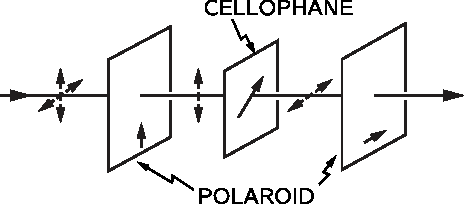
\includegraphics[width=1\linewidth]{fyz_fig0272.pdf}
      \caption{Experimentální demonstrace dvojlomu celofánu. Vektory intenzity elektrického pole
               světla jsou znázorněny čárkovaně. Směr propustnosti polaroidů a optická osa celofánu
               jsou naznačeny šipkami. Dopadající paprsek není polarizovaný.
               (\cite[s.~427]{Feynman01})}
      \label{fyz:fig0272}
    \end{figure}

    Podívejme se, co můžeme očekávat, prosvítíme-li desku z dvojlomné látky polarizovaným světlem.
    Je-li světlo polarizováno podél optické osy, projde deskou určitou rychlostí; je-li polarizováno
    kolmo, přenáší se jinou rychlostí. Zajímavá situace nastane, je-li světlo polarizováno pod úhlem
    \ang{45} k optické ose. Před chvílí jsme si řekli, že polarizace pod úhlem \ang{45} znamená
    superpozici polarizací \(x\) a \(y\) se stejnou amplitudou a fází, jak je na obr.
    \ref{fyz:fig0271a}. Protože polarizace \(x\) a \(y\) se v látce šíří různou rychlostí, jejich
    fáze se při průchodu látkou mění nestejně. Takže, i když jsou oscilace \(x\) a \(y\) na začátku
    ve fázi, v látce je fázový rozdíl mezi nimi úměrný tloušťce vrstvy. S postupem světla látkou se
    mění jeho polarizace, jak je znázorněno na sérii obrázků (obr. \ref{fyz:fig0271}). Je-li tloušťka
    desky taková, že mezi polarizacemi \(x\) a \(y\) vznikne fázový rozdíl \ang{90} jako na obr.
    \ref{fyz:fig0271c}, vyjde světlo jako kruhově polarizované. Taková destička se nazývá
    čtvrtvlnová, protože posune polarizace \(x\) a \(y\) fázově o čtvrtinu periody. Projde-li
    lineárně polarizované světlo čtvrtvlnovými destičkami, vyjde opět jako lineárně polarizované,
    ale pod pravým úhlem k původnímu směru, jak je vidět z obr. \ref{fyz:fig0271e}.

    Tento jev lze snadno znázornit kouskem celofánu. Celofán se skládá z dlouhých vláknitých molekul
    a není izotropní, neboť vlákna leží většinou vjednom směru. K demonstraci dvojlomu potřebujeme
    svazek lineárně polarizovaného světla; můžeme ho získat tak, že necháme procházet nepolarizované
    světlo vrstvou polaroidu. Polaroid (podrobně si ho probereme později) má tu užitečnou vlastnost,
    že propouští světlo lineárně polarizované podél osy polaroidu, zatímco světlo polarizované ve
    směru kolmém na osu polaroidu silně absorbuje. Propustíme-li polaroidem nepolarizované světlo,
    projde jím pouze ta část nepolarizovaného svazku, která osciluje rovnoběžně s osou polaroidu,
    takže propuštěný svazek je lineárně polarizován. Tato vlastnost polaroidu je vhodná i k detekci
    směru polarizace lineárně polarizovaného svazku nebo také k určení toho, zdaje svazek lineárně
    polarizován nebo ne. Světlo necháme prostě procházet polaroidem, přičemž jím otáčíme v rovině
    kolmé ke svazku. Je-li svazek lineárně polarizován, neprojde destičkou polaroidu, pokud je jeho
    osa kolmá ke směru polarizace. Otočíme-li polaroid o \ang{90}, projde svazek jen málo oslaben.
    Nezávisí-li intenzita procházeného světla na orientaci polaroidu, znamená to, že svazek není
    lineárně polarizován.

    K demonstraci dvojlomu celofánu použijeme dva polaroidy, jak je znázorněno na obr.
    \ref{fyz:fig0272}. První polaroid nám dává lineárně polarizovaný svazek, jenž prochází celofánem
    a pak druhým polaroidem, který nám ukáže, jak celofán ovlivnil jím procházející polarizované
    světlo. Nastavíme-li osy obou polaroidů zpočátku vzájemně kolmo a celofán odstraníme, neprojde
    druhým polaroidem žádné světlo. Vložíme-li nyní mezi polaroidy celofán a začneme jím otáčet
    kolem osy svazku, zjistíme, že část světla druhým polaroidem prochází. Existují však dva
    navzájem kolmé směry orientace celofánu, kdy druhým polaroidem neprojde žádné světlo. Tyto
    směry, při nichž celofán neovlivní jím procházející lineárně polarizované světlo, musí být
    rovnoběžně a kolmé na optickou osu celofánu.

    Předpokládáme, že při těchto dvou orientacích celofánu má světlo různou rychlost, ale směr jeho
    polarizace se nezmění. Po pootočení celofánu do střední polohy mezi těmito dvěma směry, jak je
    ukázáno na obr. \ref{fyz:fig0272}, vidíme, že druhým polaroidem prochází jasné světlo.

    Shodou okolností má celofán, jenž se běžně používá k balení, tloušťku, která je přibližně
    rovna polovině vlnové délky pro většinu barev bílého světla. Svírá-li dopadající lineárně
    polarizované světlo s optickou osou úhel \ang{45}, otočí takový celofán jeho polarizaci o
    \ang{90} a svazek vyletující z celofánu pak kmitá ve správném směru, aby mohl projít druhým
    polaroidem.

    Provedeme-li pokus s bílým světlem, bude mít celofán správnou půlvlnovou tloušťku jen pro
    některou složku bílého světla a vyletující svazek bude mít barvu této složky. Barva světla bude
    záviset na tloušťce celofánu, jíž světlo prošlo. Tuto tloušťku můžeme snadno měnit jeho
    nakláněním, takže světlo celofánem prochází šikmo, a tedy podél delší dráhy. S náklonem celofánu
    se mění barva procházejícího světla. Pomocí celofánu různých tlouštěk lze zkonstruovat filtry,
    které propouštějí různé barvy. Tyto filtry mají zajímavou vlastnost, že jsou-li osy polaroidů na
    sebe kolmé, propouštějí jednu barvu a jsou-li navzájem rovnoběžné, propouštějí doplňkovou barvu.

    Také další využití látek s uspořádanými molekulami má praktický význam. Některé plastické hmoty
    se skládají z velmi dlouhých, komplikovaných a navzájem propletených molekul. Nechá-li se
    plastická hmota opatrně ztvrdnout, uspořádají se všechny molekuly tak, že vjednom i druhém směru
    jejich stejný počet a plastická hmota není příliš dvojlomná. Při tvrdnutí působí na hmotu
    Obyčejně tlaky a mechanická napětí, takže materiál není zcela homogenní. Působíme-li na takovou
    plastickou hmotu mechanickým napětím, jako bychom tahali celou spleť vláken a ve směru
    působícího napětí bude uspořádáno více vláken než v jiných směrech. Proto, když se na určité
    plastické látky působí tlakem, stávají se dvojlomnými, jak můžeme zjistit, když je prosvítíme
    polarizovaným světlem. Při pozorování světla polaroidem je vidět soustava tmavých a světlých
    proužků, (barevných, když jsme použili bílé světlo). Při změně mechanického napětí se soustava
    proužků mění a z jejich tvaru a hustoty lze určit, jak je vzorek namáhán. V inženýrské praxi se
    ten- to jev používá k určování namáhání součástek složitých tvarů, jež by bylo možné těžko
    vypočítat.

    Jiná zajímavá možnost, jak vyvolat dvojlom je použití tekutých látek. Mějme tekutinu složenou z
    dlouhých asymetrických molekul, které mají na koncích kladný nebo záporný náboj, takže se
    chovají jako elektrické dipóly. Za normálních Okolností jsou molekuly v důsledku srážek
    orientovány náhodně a se stejným počtem molekul natočených tím nebo jiným směrem. Přiložíme-li
    elektrické pole, budou mít molekuly tendenci se uspořádat a v tom okamžiku se tekutina stane
    dvojlomnou. Se dvěma polaroidy a s průhlednou nádobkou Obsahující takovou polarizovanou tekutinu
    můžeme sestrojit zařízení, které bude propouštět světlo jen tehdy, bude-li zapnuto elektrické
    pole. Získáme tak elektrickou uzávěrku světla, jíž se také říká \textbf{Kerrův článek}.  Jev, že
    elektrické pole může v určitých tekutinách vyvolat dvojlom, se nazývá \textbf{Kerrův jev}.
  
  \section{Polarizátory}\label{fyz:IchapXXXIIIsecIV}
    Zatím jsme uvažovali látky, jež mají rozdílné indexy lomu pro světlo polarizované v různých
    směrech. Velký praktický význam mají také krystaly a jiné látky, jež mají nejen rozdílné indexy
    lomu pro světlo polarizované v různých směrech, ale i koeficienty absorpce. Na základě stejných
    důvodů, které jsme uvedli u dvojlomu, je pochopitelné, že v anizotropní látce se i absorpce může
    měnit podle směru, v němž jsou náboje nuceny kmitat. Dávno známým příkladem je turmalín a dalším
    je polaroid. Polaroid je tvořen tenkou vrstvou malých, rovnoběžně uložených krystalků
    \emph{herapathitu} (\emph{jodosulfátu chininu}). Tyto krystaly absorbují světlo oscilující v
    jednom směru a téměř neabsorbují světlo oscilující v druhém směru.
  
    \begin{figure}[ht!] %\ref{fyz:fig0273}
      \centering
      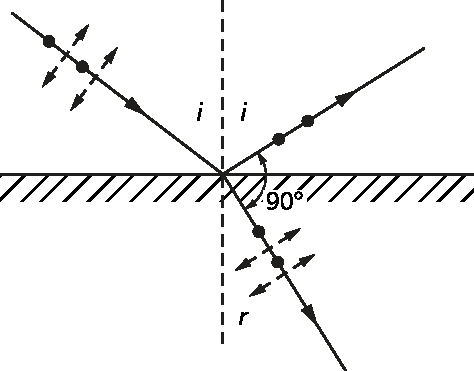
\includegraphics[width=1\linewidth]{fyz_fig0273.pdf}
      \caption{Odraz lineárně polarizovaného světla pod Brewsterovým úhlem. Směr polarizace je
               naznačen pomocí čárkovaných šipek. Kroužky znázorňují polarizaci kolmou na směr
               papíru (\cite[s.~427]{Feynman01})}
      \label{fyz:fig0273}
    \end{figure}

    Předpokládejme, že polaroid osvětlíme světlem lineárně polarizovaným pod úhlem \(\varTheta\) k
    propustnému směru. Jaká bude intenzita světla, které jde polaroidem? Dopadající světlo lze
    rozložit na složku kolmou k propustnému směru, úměrnou \(\sin\varTheta\) a na složku rovnoběžnou
    s propustným směrem, úměrnou \(\cos\varTheta\). Polaroidem pro jde jen složka amplitudy
    \(\cos\varTheta\); složka \(\sin\varTheta\) se absorbuje. Amplituda světla, jež prošlo
    polaroidem, je menší než amplituda dopadajícího světla o faktor \(\cos\varTheta\). Energie, tj.
    intenzita světla, je úměrná druhé mocnině \(\cos\varTheta\). Tedy intenzita propuštěného světla,
    je-li dopadající světlo polarizováno pod úhlem \(\varTheta\), je úměrná \(\cos^2\varTheta\).
    Intenzita absorbovaného světlaje, samozřejmě úměrná \(\sin^2\varTheta\).

    Zajímavý paradox nastane za takovéto situace: Víme, že dvěma zkříženými polaroidy, jejichž osy
    svírají pravý úhel, svazek světla neprochází. Vsuneme-li však \emph{mezi} oba polaroidy destičku
    třetího polaroidu s osou propustnosti pod úhlem \ang{45} k osám zkřížených polaroidů, nějaké
    světlo projde. Víme, že polaroid světlo nevytváří, ale absorbuje ho. Přesto přidání třetího
    polaroidu pod úhlem \ang{45} umožní nějakému světlu proletět. Analýzu tohoto jevu ponecháme
    čtenáři jako cvičení.

    Jeden z nejzajímavějších příkladů polarizace nenastává u komplikovaných krystalů nebo složitých
    látek, ale při jednom z nejznámějších a nejjednodušších jevů - při odrazu světla od povrchu.
    Věřte nebo ne, světlo odražené od povrchu skla může být polarizované a lze to velmi snadno
    fyzikálně vysvětlit. Brewster experimentálně zjistil, že světlo odražené od povrchu je úplně
    polarizované, svírají-li odražený a lomený paprsek v látce pravý úhel. Tato situace je
    znázorněna na obr. \ref{fyz:fig0273}. Je-li dopadající paprsek polarizován v rovině dopadu, odraz
    vůbec nenastane. Paprsek se odrazí pouze tehdy, je-li dopadající paprsek polarizován kolmo k
    rovině dopadu. Důvod lze velmi snadno pochopit. V látce je světlo polarizováno příčně a víme, že
    jsou to právě pohyby nábojů, jež generují vynořující se paprsek, který nazýváme odraženým.
    Zdrojem tohoto odraženého světla není prostě odraz dopadajícího paprsku. Hlubší analýza tohoto
    jevu nám říká, že dopadající paprsek rozkmitá v látce náboje, které pak generují odražený
    paprsek. Z obr. \ref{fyz:fig0273} je jasné, že jen kmity kolmé na rovinu papíru mohou vyzařovat
    ve směru odrazu a proto odražený paprsek bude polarizován kolmo na rovinu dopadu. Je-li
    dopadající paprsek polarizován v rovině dopadu, žádné světlo se neodrazí.

    Tento jev lze jasně ukázat na odrazu lineárně polarizovaného světla dopadajícího na kousek
    plochého skla. Nastavením skla pod různými úhly dopadu pro polarizovaný paprsek je možné Zjistit
    náhlý pokles intenzity odraženého světla právě při dopadu pod \textbf{Brewsterovým úhlem}. Tento
    pokles je vidět jen tehdy, leží-li rovina polarizace v rovině dopadu.je-li kolmá k rovině
    dopadu, pozorujeme obvyklou intenzitu odraženého světla ve všech směrech.

  \section{Optická aktivita}\label{fyz:IchapXXXIIIsecV}
    Další velmi zajímavý polarizační jev můžeme pozorovat v látkách složených z molekul bez
    zrcadlové symetrie: u molekul ve tvaru vývrtky nebo ve tvaru rukavice či jakéhokoliv jiného
    tvaru, který se v zrcadle zobrazuje tak, jako když levá rukavice přechází v pravou.
    Předpokládejme, že všechny molekuly v látce jsou stejného typu, tj. žádná není zrcadlovým
    obrazem druhé. U takové látky se může projevovat zvláštní jev, nazvaný \emph{optická aktivita},
    kdy lineárně polarizované světlo, které touto látkou prochází, stáčí směr polarizace kolem osy
    paprsku.
  
    \begin{figure}[ht!] %\ref{fyz:fig0274}
      \centering
      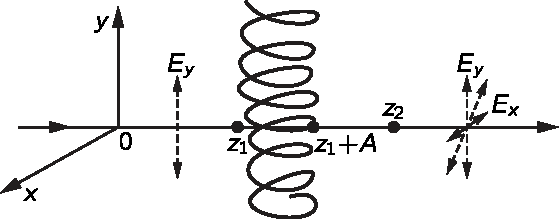
\includegraphics[width=1\linewidth]{fyz_fig0274.pdf}
      \caption{Tvar molekuly, která nemá zrcadlovou symetrii. Na molekulu dopadá světelný paprsek
              lineárně polarizovaný ve směru osy \(y\). (\cite[s.~427]{Feynman01})}
      \label{fyz:fig0274}
    \end{figure}

    K pochopení optické aktivity jsou potřebné určité výpočty, ale i bez nich můžeme kvalitativně
    ukázat, jak tento jev vzniká. Vezměme asymetrickou molekulu spirálovitého tvaru, jaká je
    Znázorněna na obr. \ref{fyz:fig0274}. K tomu, aby se u látky projevila optická aktivita, není
    nutné, aby její molekuly měly tvar vývrtky, ale tento jednoduchý tvar si vezmeme jako typický
    příklad pro molekuly bez zrcadlové symetrie. Dopadá-li na molekulu světlo lineárně polarizované
    ve směru osy \(y\), jeho elektrické pole rozkmitá náboje podél závitů spirály, čímž vytvoří
    proud ve směru osy \(y\) a náboje budou vyzařovat elektrické pole \(E_y\), polarizované v ose
    \(y\). Jsou-li elektrony při kmitání nuceny se pohybovat podél spirály, musí se pohybovat také
    ve směru osy \(x\). Proud procházející podél spirály vtéká v bodě \(z=z_1\) do roviny papíru a v
    bodě \(z=z_1 + A\) ven z papíru (\(A\) je průměr naší spirálové molekuly). Lze předpokládat, že
    proud ve směru osy \(x\) nevyvolá žádné výsledné záření, neboť na protilehlých stranách spirály
    teče opačným směrem. Vezmeme-li však složku pole \(x\) v bodě \(z=z_2\), vidíme, že pole
    vyzářené proudem z bodu \(z=z_1 + A\) a pole z bodu \(z=z_1\) se dostanou do bodu \(z_2\) s
    časovým rozdílem \(A/c\), takže jejich fázový posun je \(\pi + \omega A/c\). Protože tento
    fázový rozdíl není roven přesně \(\pi\), tato dvě pole se úplně neruší a zůstane nám malá složka
    \(x\) elektrického pole vytvořeného pohybem elektronů v molekule, zatímco budící elektrické pole
    mělo jen složku \(y\). Součet této malé složky \(x\) a velké složky \(y\) vytváří výsledné pole,
    jež je mírně skloněno vzhledem k ose \(y\), tj. k původnímu směru polarizace, jak světlo
    postupuje látkou, směr jeho polarizace se otáčí kolem osy paprsku. Pomocí několika dalších
    příkladů a analýzou proudů indukovaných dopadajícím elektrickým polem lze ukázat, že existence
    optické aktivity a znaménko rotace jsou nezávislé na orientaci molekul.

    Běžnou látkou, jež se vyznačuje optickou aktivitou, je glukosa. Lze to snadno ukázat pomocí
    polaroidové destičky, která vytvoří lineárně polarizovaný paprsek, průhledné nádobky obsahující
    glukosu a druhé destičky, jíž se zjistí pootočení směru polarizace při průchodu světla glukosou.

  \section{Intenzita odraženého světla}\label{fyz:IchapXXXIIIsecVI}
    Nyní se podívejme na koeficient Odrazu jako na funkci úhlu. Obrázek \ref{fyz:fig0275a}. znázorňuje
    dopad světelného paprsku na povrch skla, kde se částečně odráží a částečně láme směrem do skla.
    Nechť je dopadající paprsek jednotkové amplitudy lineárně polarizovaný kolmo na rovinu papíru.
    Amplitudu odraženého světla označíme \(b\) a amplitudu lomeného paprsku \(a\). Samozřejmě, že
    odražený i lomený paprsek budou lineárně polarizované a vektory intenzit elektrického pole
    dopadající, budou odražené a lomené vlny navzájem rovnoběžné. Obrázek \ref{fyz:fig0275b}
    znázorňuje stejnou situaci, ale teď' předpokládáme, že dopadající vlna jednotkové amplitudy je
    polarizována v rovině papíru. Amplitudy odražené a lomené vlny si nyní označme jako \(A\) a
    \(B\).
  
    \begin{figure}[ht!]  %\ref{fyz:fig0275}
      \centering
      \subcaptionbox{\label{fyz:fig0275a}}{\luafigure[0.45]{fyz_fig0275a.pdf}}
      \subcaptionbox{\label{fyz:fig0275b}}{\luafigure[0.45]{fyz_fig0275b.pdf}}
      \caption{Odraz a lom vlny s jednotkovou amplitudou dopadající na povrch skla. a) Dopadající
              vlna je lineárně polarizovaná kolmo na rovinu papíru. b) Dopadající vlna je lineárně
              polarizovaná ve směru znázorněném čárkovaným vektorem intenzity elektrického pole.      
              (\cite[s.~437]{Feynman01})}
      \label{fyz:fig0275}
    \end{figure}

  \section{Anomální lom světla}\label{fyz:IchapXXXIIIsecVIII}

    \begin{figure}[ht!]  %\ref{fyz:fig0276}
      \centering
      \subcaptionbox{\label{fyz:fig0276a}}{\luafigure[0.8]{fyz_fig0276a.pdf}} \\
      \subcaptionbox{\label{fyz:fig0276b}}{\luafigure[0.8]{fyz_fig0276b.pdf}}
      \caption{Obrázek vlevo znázorňuje dráhu řádného paprsku při průchodu dvojlomným krystalem.
              Mimořádný paprsek je znázorněn na obrázku vpravo. Optická osa leží v rovině papíru.
              (\cite[s.~437]{Feynman01})}
      \label{fyz:fig0276}
    \end{figure}

    
    \begin{figure}[ht!] %\ref{fyz:fig0277}
      \centering
      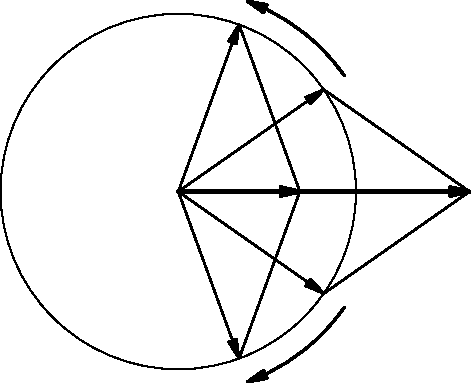
\includegraphics[width=0.6\linewidth]{fyz_fig0277.pdf}
      \caption{Součet dvou vektorů se stejnou amplitudou rotujících v opačných směrech dává vektor
               oscilující podél pevně přímky. (\cite[s.~427]{Feynman01})}
      \label{fyz:fig0277}
    \end{figure}
    
    \begin{figure}[ht!] %\ref{fyz:fig0278}
      \centering
      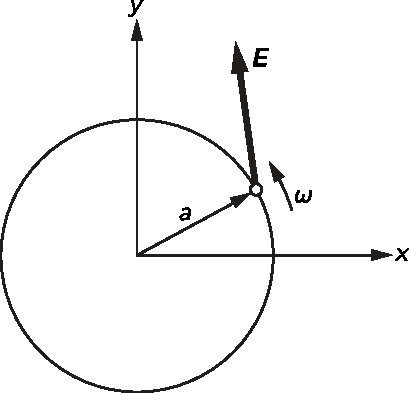
\includegraphics[width=0.6\linewidth]{fyz_fig0278.pdf}
      \caption{Pohyb náboje po kružnici vyvolaný kruhově polarizovaným světlem.
               (\cite[s.~427]{Feynman01})}
      \label{fyz:fig0278}
    \end{figure}

  \section{Příklady a cvičení}\label{fyz:IchapXXXIIIsecIX}

%---------------------------------------------------------------------------------------------------